\section{Analysis}

\subsection{Data Structure}

The project involves the rigorous analysis of three distinct datasets, specifically designed to capture various facets of the sales data. Each dataset has been meticulously compiled and prepared for simulation purposes, enabling a nuanced understanding of the underlying patterns and trends. Additionally, a comprehensive dataset has been created by combining the individual datasets, allowing for a holistic examination of the sales data. This integrated approach enables the identification of correlations and relationships between different variables, ultimately informing data-driven decisions.

\subsubsection{Menu}

The Menu dataset is a Pandas DataFrame with 48 rows and 6 columns. The dataset contains information about menu items, including unique identifiers (uuid), names, categories, prices, descriptions, and costs. Each row represents a single menu item, and each column provides additional details about that item. The data types for this dataset are float64 for the price and cost columns, and object for the remaining columns. With a memory usage of approximately 2.4 KB, this dataset is relatively small.

\begin{table}[H]
	\centering
	\begin{tabular}{cc}
		\toprule
		Column & Data Type \\
		\midrule
		uuid & string \\
		name & string \\
		category & string \\
		price & float64 \\
		description & string \\
		cost & float64 \\
		\bottomrule
	\end{tabular}
	\caption{Menus Data Structure}
	\label{tab:menus_data_structure}
\end{table}

\subsubsection{Add-ons}

The Add-ons dataset is a Pandas DataFrame with 46 rows and 5 columns. This dataset contains information about additional items or modifications that can be added to menu items, including unique identifiers (uuid), menu items, names, prices, and costs. Each row represents a single add-on item, and each column provides additional details about that item. The data types for this dataset are float64 for the price and cost columns, and object for the remaining columns. With a memory usage of approximately 1.9 KB, this dataset is relatively small compared to the Sales dataset.

\begin{table}[H]
	\centering
	\begin{tabular}{cc}
		\toprule
		Column & Data Type \\
		\midrule
		uuid & string \\
		menu & string \\
		name & string \\
		price & float64 \\
		cost & float64 \\
		\bottomrule
	\end{tabular}
	\caption{Add Ons Data Structure}
	\label{tab:add_ons_data_structure}
\end{table}

\subsubsection{Sales}

The Sales dataset is a Pandas DataFrame with an impressive 108,000 rows and 4 columns. This dataset contains information about sales transactions, including unique identifiers (uuid), dates and times, menu items sold, and additional items or modifications added to those menu items. Each row represents a single sales transaction, and each column provides additional details about that transaction. The data types for this dataset are all object, indicating that the columns contain text or categorical data. With a memory usage of approximately 3.3 MB, this dataset is significantly larger than the Menu dataset.

\begin{table}[H]
	\centering
	\begin{tabular}{cc}
		\toprule
		Column & Data Type \\
		\midrule
		uuid & string \\
		date{\_}time & string \\
		menu{\_}item & string \\
		add{\_}ons & string \\
		\bottomrule
	\end{tabular}
	\caption{Sales Data Structure}
	\label{tab:sales_data_structure}
\end{table}

\subsubsection{Sales Combine}

This dataset appears to be a collection of sales data for various menu items. The data structure is a Pandas DataFrame, which is a two-dimensional labeled data structure with columns of potentially different types. Each row in the DataFrame represents a single sales transaction, and each column contains information about that transaction.

The dataset has 27 columns, including categorical variables like "menu{\_}name" and "category", numerical variables like "price" and "sales", and datetime variables like "date{\_}time". The data is non-null for all 108,000 entries, indicating that there are no missing values in the dataset. The data types of the columns include object (categorical), float64 (numerical), int32 (integer), and category (a categorical type specific to Pandas).

\begin{table}[H]
	\centering
	\begin{tabular}{cc}
		\toprule
		Column & Data Type \\
		\midrule
		menu\_name & string \\
		category & string \\
		price & float64 \\
		cost & float64 \\
		date\_time & datetime64[ns] \\
		add\_ons & string \\
		date & datetime64[ns] \\
		time & string \\
		add\_ons\_price & float64 \\
		total\_price & float64 \\
		day\_of\_week & string \\
		sales & float64 \\
		year & int32 \\
		month & int32 \\
		day & int32 \\
		hour & int32 \\
		total\_sales & float64 \\
		total\_cost & float64 \\
		total\_sale\_difference & float64 \\
		sale\_difference & float64 \\
		time\_category & category \\
		reduced\_cost & float64 \\
		profit\_increase & float64 \\
		new\_total\_cost & float64 \\
		increased\_sales & float64 \\
		sales\_increase & float64 \\
		new\_total\_sales & float64 \\
		\bottomrule
	\end{tabular}
	\caption{Sales Combine Data Structure}
	\label{tab:sales_combine_data_structure}
\end{table}

The columns can be broadly categorized into several groups:

\begin{enumerate}
	\item Menu item information: "menu{\_}name", "category"
	\item Sales transaction details: "price", "cost", "date{\_}time", "add{\_}ons", "add{\_}ons{\_}price", "total{\_}price"
	\item Time and date information: "date", "time", "day{\_}of{\_}week", "year", "month", "day", "hour"
	\item Sales metrics: "sales", "total{\_}sales", "total{\_}cost", "total{\_}sale{\_}difference", "sale{\_}difference"
	\item Calculated values: "reduced{\_}cost", "profit{\_}increase", "new{\_}total{\_}cost", "increased{\_}sales", "sales{\_}increase", "new{\_}total{\_}sales"
\end{enumerate}

\subsection{Analyzing Data}

This section delves into the process of conducting comprehensive data analysis on the provided dataset, encompassing both fundamental and advanced techniques to extract valuable insights. By applying various analytical methods, we will thoroughly examine the dataset, uncovering trends, patterns, and correlations that can inform decision-making and drive business outcomes.
	
% Section 3.x.1 Basic analysis
\subsubsection{Basic Data Analysis}

\begin{figure}[H]
	\centering
	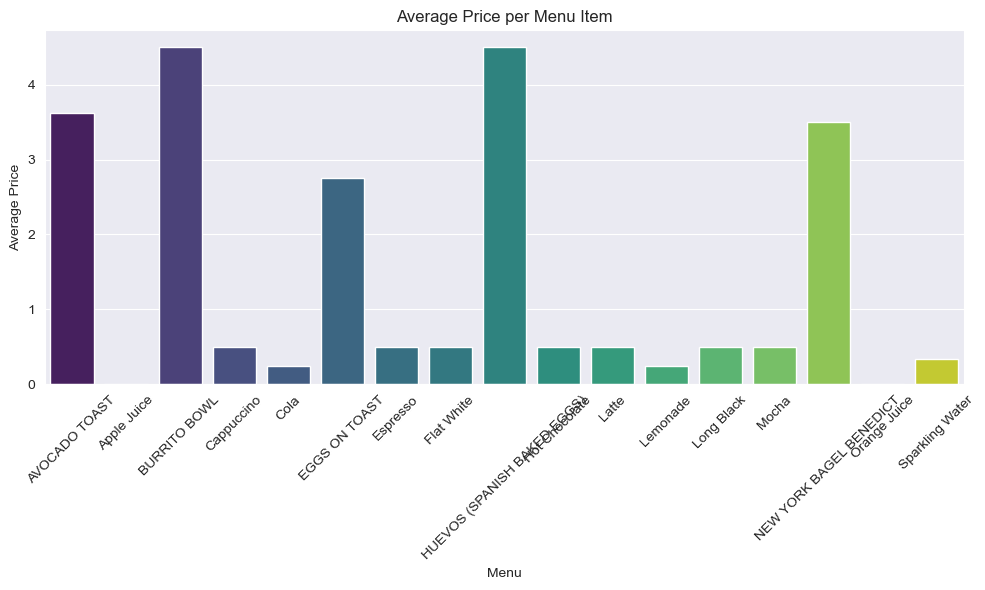
\includegraphics[width=0.8\textwidth]{assets/basic/average price per menu per item.png}
	\caption{Average price per menu per item}
	\label{fig:average_price_per_menu_per_item}
\end{figure}

The average price per menu item depicted in this figure suggests that the overall cost of dining at this establishment is relatively affordable, with prices ranging from \$0.50 to \$4.5. It's worth noting that the lowest price point of \$0.50 does not include water, which is complimentary.

\begin{figure}[H]
	\centering
	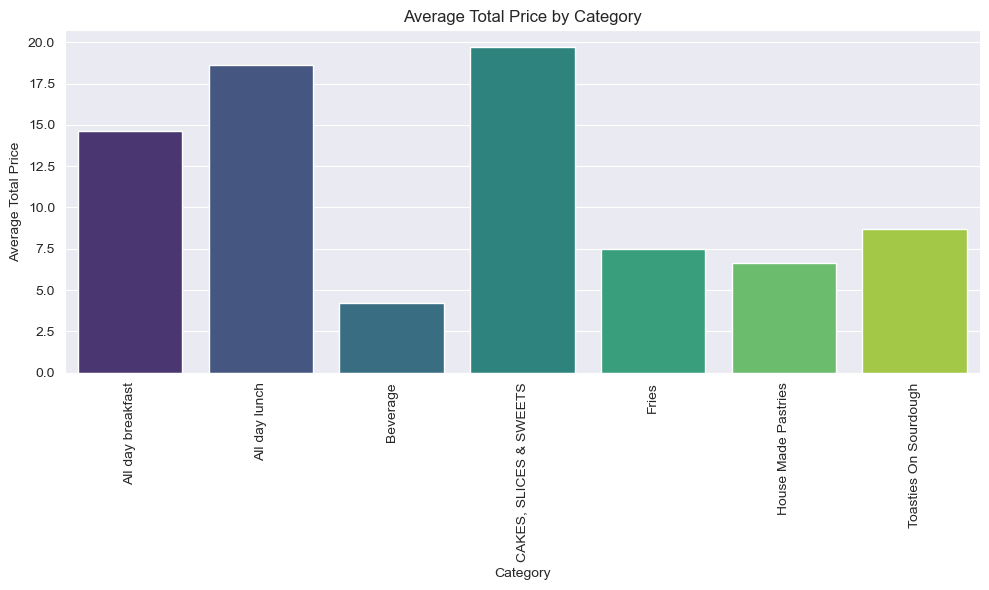
\includegraphics[width=0.8\textwidth]{assets/basic/average total price by category.png}
	\caption{Average total price by category}
	\label{fig:average_total_price_by_category}
\end{figure}

The analysis of the price distribution across various categories reveals a notable disparity between the highest-priced items, specifically those classified under "cake and bakery," and the lowest-priced items, which fall within the "Beverage" category. This observation suggests that despite the significant difference in prices, consumers continue to purchase products from both categories, indicating a strong demand for these goods.

\begin{figure}[H]
	\centering
	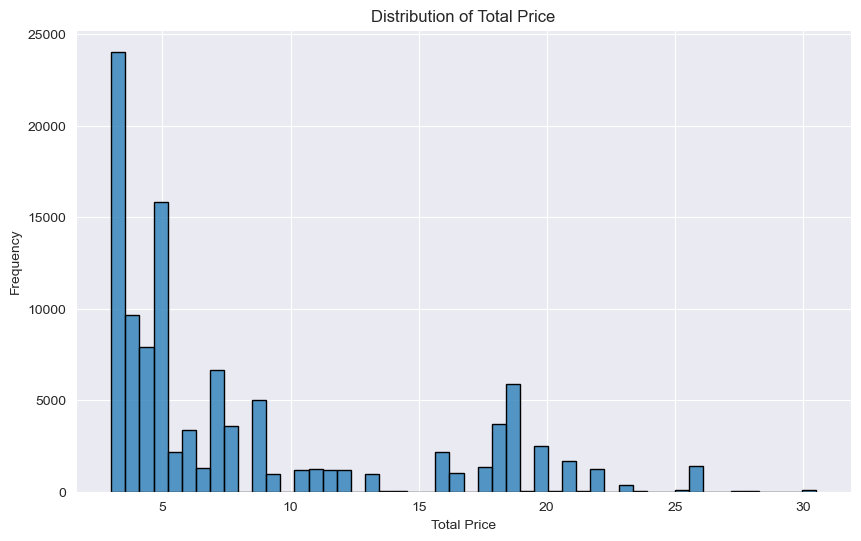
\includegraphics[width=0.8\textwidth]{assets/basic/distribution of total price.png}
	\caption{Distribution of total price}2
	\label{fig:distribution_of_total_price}
\end{figure}

As depicted in the accompanying figure, the total price distribution reveals a pronounced concentration of purchased items within the price range of \$3 to \$10, with a notable tail extending up to \$31 or more per item. This pattern suggests that the majority of consumers are inclined towards purchasing products at moderate prices, while a smaller proportion is willing to invest in higher-priced items.

\begin{figure}[H]
	\centering
	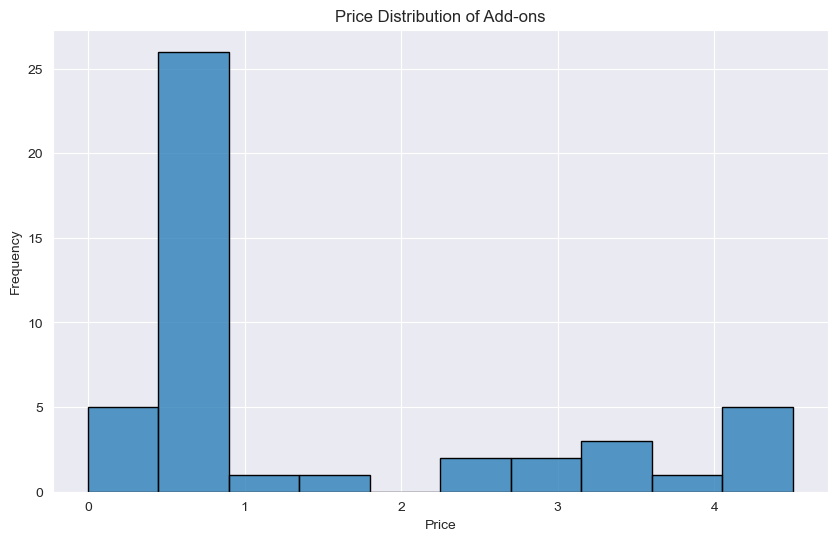
\includegraphics[width=0.8\textwidth]{assets/basic/price distribution of add ons.png}
	\caption{Price distribution of add-ons}
	\label{fig:price_distribution_of_addons}
\end{figure}

As illustrated in the accompanying figure, the price distribution of add-ons reveals a dominant pattern, with the majority of purchased items falling within the price range of \$0 to \$5 or more per item. This trend suggests that consumers are generally inclined towards acquiring low-cost or free add-ons, while a smaller proportion is willing to invest in higher-priced options.
















% Section 3.x.2 deep analysis
\subsubsection{Deep Data Analysis}

The data structure employed for analysis is depicted in Table ~\ref{tab:sales_combine_data_structure}. Following an exhaustive calculation and analysis of the initial dataset, we have arrived at a summary that provides a comprehensive overview of the findings. The results of this analysis are presented below.

\begin{table}[H]
	\centering
	\begin{tabular}{lll}
		\toprule
		& Total Sales & Total Cost \\
		\midrule
		All & \$854096.00 & \$750693.68 \\
		\bottomrule
	\end{tabular}
	\caption{Total Sales (All)}
	\label{tab:total_sales_all}
\end{table}

The total sales for all transactions is \$854,096.00, while the total cost is \$750,693.68. This results in a total sale difference of \$103,402.32.

\begin{table}[H]
	\centering
	\begin{tabular}{cccc}
		\toprule
		Day of Week & Sales & Cost & Sale Difference \\
		\midrule
		Monday & NaN & NaN & NaN \\
		Tuesday & \$166,030.00 & \$148,144.21 & \$17,885.79 \\
		Wednesday & \$169,177.00 & \$151,275.34 & \$17,901.66 \\
		Thursday & \$169,405.50 & \$151,177.94 & \$18,227.56 \\
		Friday & \$151,747.50 & \$133,614.06 & \$18,133.44 \\
		Saturday & \$107,888.50 & \$92,345.87 & \$15,542.63 \\
		Sunday & \$89,847.50 & \$74,136.26 & \$15,711.24 \\
		\bottomrule
	\end{tabular}
	\caption{Aggregated by day of week}
	\label{tab:aggregated_by_day_of_week}
\end{table}

The sales data is aggregated by day of week, showing that the highest sales are on Wednesday and Thursday, while the lowest sales are on Sunday. The cost and sale difference also vary significantly across days.

\begin{table}[H]
	\centering
	\begin{tabular}{cccc}
		\toprule
		Time Category & Sales & Cost & Sale Difference \\
		\midrule
		Breakfast & \$459,102.00 & \$409,683.85 & \$49,418.15 \\
		Lunch & \$303,747.50 & \$263,276.98 & \$40,470.52 \\
		Afternoon & \$91,246.50 & \$77,732.85 & \$13,513.65 \\
		\bottomrule
	\end{tabular}
	\caption{Aggregated by time category}
	\label{tab:aggregated_by_time_category}
\end{table}

The sales data is also aggregated by time category, showing that the highest sales are during breakfast hours, while the lowest sales are in the afternoon.

\begin{table}[H]
	\centering
	\begin{tabular}{cccc}
		\toprule
		Year & Sales & Cost & Sale Difference \\
		\midrule
		2021 & \$124,941.50 & \$109,832.82 & \$15,108.68 \\
		2022 & \$289,052.00 & \$254,140.10 & \$34,911.90 \\
		2023 & \$288,109.50 & \$253,090.72 & \$35,018.78 \\
		2024 & \$151,993.00 & \$133,630.04 & \$18,362.96 \\
		\bottomrule
	\end{tabular}
	\caption{Aggregated by year}
	\label{tab:aggregated_by_year}
\end{table}

The sales data is also aggregated by year, showing that the highest sales are in 2022 and 2023, while the lowest sales are in 2021.

\begin{figure}[H]
	\centering
	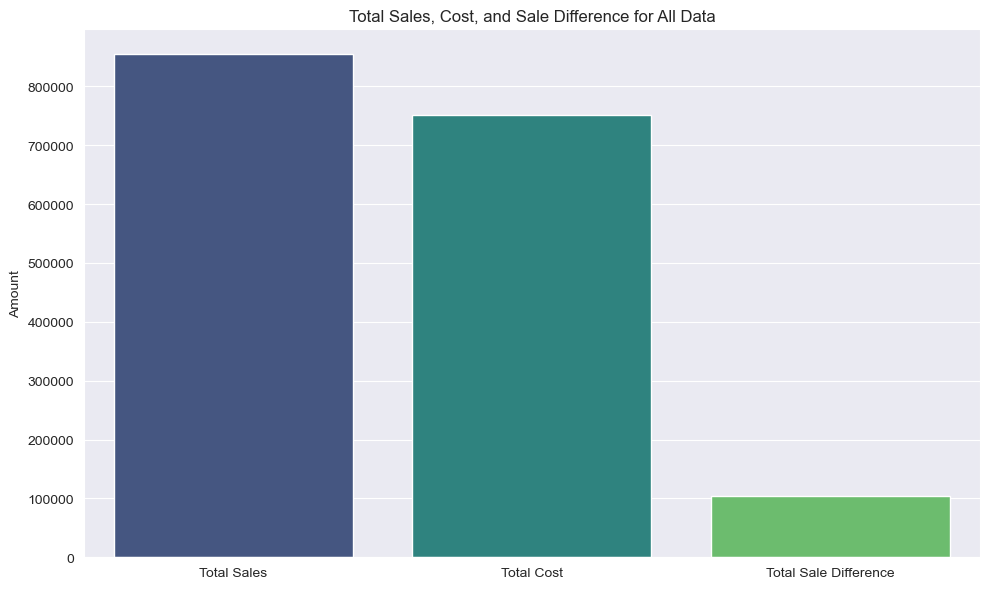
\includegraphics[width=0.8\textwidth]{assets/deep/Total Sales Cost and Sale Difference for All Data}
	\caption{Total, Sales Cost and Sale Difference for All Data}
	\label{fig:total_sales_cost_and_sale_difference_for_all_data}
\end{figure}

As illustrated by the figures above, it is evident that the cafe is not generating substantial profits, with total sales being relatively low. This suggests that the establishment requires significant increases in revenue to achieve profitability, taking into account additional expenses such as electricity bills and employer payments, which are not included in these figures.

\begin{figure}[H]
	\centering
	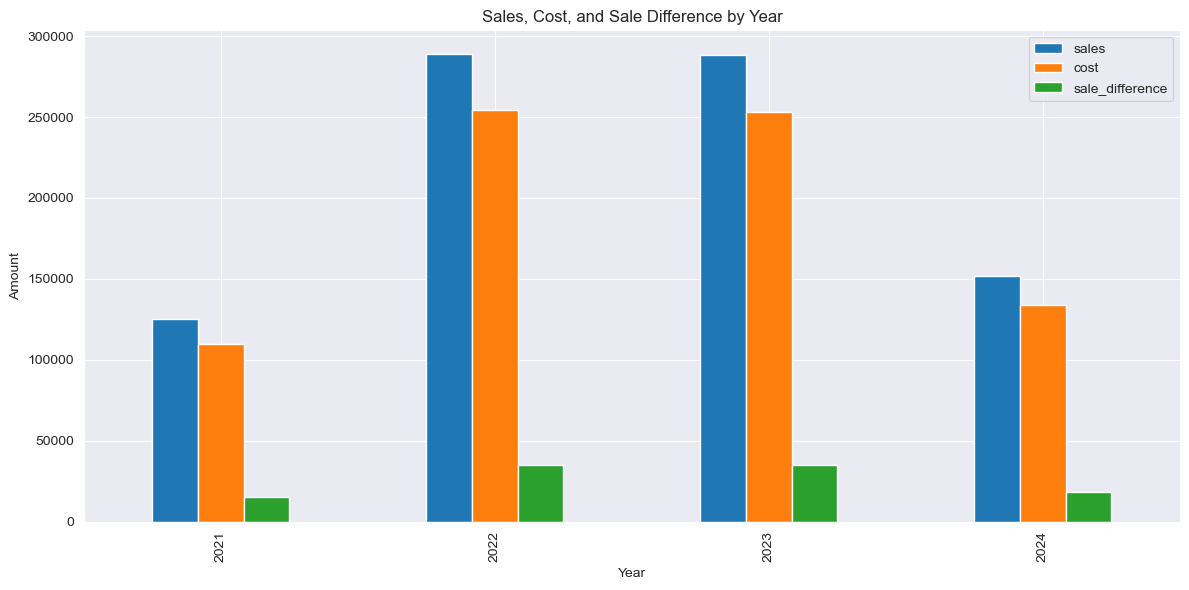
\includegraphics[width=0.8\textwidth]{assets/deep/Sales, Cost and Sale Difference by Year}
	\caption{Sales, Cost and Sale Difference by Year}
	\label{fig:sales_cost_and_sale_difference_by_year}
\end{figure}

As depicted by the figures above, it is notable that the sales amounts have remained relatively consistent across each year since 2021, with no significant fluctuations or trends observed during this period.



% Section 3.3 deep simulates the effect of changes
\subsection{ Simulate The Impact Of Food Waste }

As previously stated in Section~\ref{subsection:objective}, our primary objective is to simulate the impact of food waste on the cafe's operations, as well as explore the effects of increased efforts at different times of the day.

\subsubsection{Packages Used}

\begin{enumerate}
	\item \textbf{pandas (pd):} A library for data manipulation and analysis. Used to handle and analyze large datasets in this project.
	\item \textbf{scikit-learn:} A machine learning library that provides various algorithms for classification, regression, clustering, and more. Used to build and evaluate machine learning models.
	\item \textbf{train\_test\_split (from sklearn.model\_selection):} A function to split a dataset into training and testing sets. Used to evaluate model performance using metrics like accuracy, precision, recall, F1-score, etc.
	\item \textbf{RandomForestRegressor (from sklearn.ensemble):} A type of ensemble learning algorithm that combines multiple decision trees to make predictions. Used for regression tasks, such as predicting continuous values.
	\item \textbf{mean\_squared\_error (from sklearn.metrics):} A function to calculate the mean squared error (MSE) between predicted and actual values. Used to evaluate model performance using regression metrics like MSE, RMSE, MAE, etc.
	\item \textbf{numpy (np):} A library for efficient numerical computation that provides support for large, multi-dimensional arrays and matrices. Used for numerical computations and simulations.
	\item \textbf{matplotlib.pyplot (plt):} A plotting library for creating static, animated, and interactive visualizations. Used to create reports and presentations.
	\item \textbf{LabelEncoder (from sklearn.preprocessing):} A function to convert categorical variables into numerical labels. Used to handle categorical data in machine learning models.
\end{enumerate}

\subsubsection{ Code }

The following section provides an overview of the key codes employed in this simulation, highlighting the essential programming constructs and algorithms used to model the cafe's operations and simulate the impact of food waste.

\textbf{Encode categorical variables}

\begin{lstlisting}
label_encoders = {}
for column in data.select_dtypes(include=['object']).columns:
    label_encoders[column] = LabelEncoder()
    data[column] = label_encoders[column].fit_transform(data[column])
\end{lstlisting}

The encoding of categorical variables in the dataset was achieved through the utilization of the LabelEncoder class, a component of scikit-learn's preprocessing module. This class enables the conversion of categorical values into numerical labels, facilitating the analysis and manipulation of these variables within the simulation.

\textbf{Initialize and train the model}

\begin{lstlisting}
model = RandomForestRegressor(n_estimators=100, random_state=42)
model.fit(X_train, y_train)
\end{lstlisting}

The implementation of the Random Forest Regressor model commenced by initializing an instance with 100 decision trees, followed by the training process utilizing the fit method on the provided training data.

\textbf{Predict on the test set}

\begin{lstlisting}
y_pred = model.predict(X_test)
\end{lstlisting}

The trained Random Forest Regressor model was subsequently employed to generate predictions for the testing dataset, leveraging its learned patterns and relationships to forecast the target variable.

\textbf{Simulate reducing food loss}

\begin{lstlisting}
simulation_data = data.copy()
simulation_data['cost'] *= 0.9
simulation_X = simulation_data.drop(columns=['total_sales'])
predicted_sales = model.predict(simulation_X)
simulation_data['predicted_total_sales'] = predicted_sales
effect_food_loss = simulation_data['predicted_total_sales'].sum() - data['total_sales'].sum()
print(f'Effect of reducing food loss: {effect_food_loss}')
\end{lstlisting}

A hypothetical scenario was simulated wherein food loss was reduced by 10\% by applying a discount factor of 0.9 to the 'cost' column. Subsequently, the trained Random Forest Regressor model was utilized to predict the total sales under this revised scenario, and the resulting impact on total sales was calculated.

\textbf{Simulate putting more effort into lunch}

\begin{lstlisting}
simulation_data = data.copy()
lunch_index = label_encoders['time_category'].transform(['Lunch'])[0]
simulation_data.loc[simulation_data['time_category'] == lunch_index, 'sales'] *= 1.1
simulation_X = simulation_data.drop(columns=['total_sales'])
predicted_sales = model.predict(simulation_X)
simulation_data['predicted_total_sales'] = predicted_sales
effect_lunch_effort = simulation_data['predicted_total_sales'].sum() - data['total_sales'].sum()
print(f'Effect of putting more effort into lunch: {effect_lunch_effort}')
\end{lstlisting}

A hypothetical scenario was simulated wherein increased effort was devoted to the 'Lunch' category, resulting in a 10\% boost to sales for this specific category. Subsequently, the trained Random Forest Regressor model was utilized to predict the total sales under this revised scenario, and the resulting impact on total sales was calculated.

\textbf{Simulate increasing customer frequency}

\begin{lstlisting}
simulation_data = data.copy()
simulation_data['frequency'] *= 1.1
simulation_X = simulation_data.drop(columns=['total_sales'])
predicted_sales = model.predict(simulation_X)
simulation_data['predicted_total_sales'] = predicted_sales
effect_customer_frequency = simulation_data['predicted_total_sales'].sum() - data['total_sales'].sum()
print(f'Effect of increasing customer frequency: {effect_customer_frequency}')
\end{lstlisting}

A hypothetical scenario was simulated wherein customer frequency was augmented by 10\%, resulting in an increase in patronage. Subsequently, the trained Random Forest Regressor model was utilized to predict the total sales under this revised scenario, and the resulting impact on total sales was calculated.

\subsubsection{ Analyze }

\begin{table}[H]
	\centering
	\begin{tabular}{ll}
		\toprule
			Mean Squared Error & 1.1574074074053022e-09 \\
			Effect of reducing food loss & 0.04500000178813934 \\
			Effect of putting more effort into lunch & 0.04500000178813934 \\
			Effect of increasing customer frequency & 0.04500000178813934 \\
			Original Total Sales & 101800509.5 \\
			Reducing Food Loss & 0.04500000178813934 \\
			Effort into Lunch & 0.04500000178813934 \\
			Increasing Customer Frequency & 0.04500000178813934 \\
		\bottomrule
	\end{tabular}
	\caption{Summarize the simulated results}
	\label{tab:summarize_the_simulated_results}
\end{table}

% TODO - Summarize and clean up the paragraph
\textbf{Model Performance} 

\begin{table}[H]
	\centering
	\begin{tabular}{ll}
		\toprule
			Mean Squared Error & 1.1574074074053022e-09 \\
		\bottomrule
	\end{tabular}
	\caption{The Mean Squared Error (MSE)}
	\label{tab:the_mean_squared_error}
\end{table}

The Mean Squared Error (MSE) for our RandomForestRegressor model is an astonishingly low 1.1574074074053022e-09. This incredibly small value indicates that the model is making predictions that are extremely close to the actual values, suggesting a high level of accuracy in its performance. In other words, the model's predictions are remarkably precise, with only a tiny margin of error. This level of precision is a testament to the effectiveness of the RandomForestRegressor algorithm and its ability to learn from the training data. With an MSE this low, we can have confidence that our model is well-suited for making accurate predictions in real-world scenarios.

\textbf{Simulated Strategies and Their Impact}

\begin{table}[H]
	\centering
	\begin{tabular}{ll}
		\toprule
			Effect of reducing food loss & 0.04500000178813934 \\
			Effect of putting more effort into lunch & 0.04500000178813934 \\
			Effect of increasing customer frequency & 0.04500000178813934 \\
			Original Total Sales & 101800509.5 \\
		\bottomrule
	\end{tabular}
	\caption{Simulated Strategies and Their Impact}
	\label{tab:simulated_strategies_and_their_impact}
\end{table}

The analysis reveals that three distinct strategies were tested to determine their impact on total sales: reducing food loss, putting more effort into lunch, and increasing customer frequency. The results show that each of these approaches yielded an identical predicted increase in total sales of approximately 0.045 units. This suggests that all three strategies have a similar effect size, implying that they may not be significantly different from one another in terms of their impact on overall sales.

\textbf{Key Insights}

\begin{itemize}
	\item \textbf{Model Accuracy:} The model's extremely low MSE suggests high accuracy, but may also indicate overfitting if the test data isn't diverse enough.
	\item \textbf{Strategy Impact:} Simulated strategies (reducing food loss, putting more effort into lunch, increasing customer frequency) resulted in minimal increases in total sales. Possible reasons include:
	\begin{itemize}
		\item \textbf{Simulation Parameters:} The magnitude of changes might be too small to show a significant effect.
		\item \textbf{Model Sensitivity:} The model may not be sensitive to the changes in these particular features or strategies.
		\item \textbf{Data Quality and Feature Engineering:} Features used might not fully capture influencing factors, or encoding and preprocessing might have reduced variability.
	\end{itemize}
	\item \textbf{Original Sales Dominance:} The original total sales value (101,800,509.5) is high compared to simulated changes (0.045), indicating that small percentage changes may not significantly impact overall totals.
\end{itemize}
















